\section{Recovered observation vintages and calibration tests}
\subsection{What the written calibration specification now supplies}
The later Darnell manuscript's supplementary Table 2\cite{darnell2025} identifies HadCRUT5.0.1.0
temperature for 1850--2021, Law Dome CO$_2$ for 1854--1953, Mauna Loa CO$_2$ for
1959--2017, and 0--3000 m ocean heat content for 1953--1996. It also identifies
the IMBIE, glacier and global sea-level products used in the joint calibration.
This recovers several input definitions that the initial assessment treated as
missing. The later table is evidence about the methodological lineage; its
identity with the target's unpinned 2024 manuscript remains unestablished.
The 2024 text explicitly adds autoregressive residuals to simulated observables,
and Urban and Keller provide the stationary AR(1) likelihood\cite{urban}.
Neither the statistical family nor all observation versions should therefore
be described as inaccessible.

Original-provider archives supply the specified HadCRUT5 version and 83
irregular Law Dome readings within the stated period. NOAA supplies a current
Mauna Loa annual series. Its 2026 release date is recorded; it is not silently
equated with the target's historical release. Gouretski and Koltermann's
written 3000 m heat estimate is a $12.8\times10^{22}$ J increase between
1957--1966 and 1987--1996, with uncertainty of at least $8\times10^{22}$ J
\cite{gouretski}. We recover this aggregate constraint but not a verified annual
1953--1996 series. We do not digitize their curve or assign their uncertainty
statement a Gaussian standard deviation. The existing HadCRUT4/700 m posterior
predicts a median increase of $6.17\times10^{22}$ J over those decades, with a
parameter 5th--95th range of $4.86$--$12.37\times10^{22}$ J. Different depths,
error definitions and averaging conventions require explicit treatment in any
subsequent joint fit.

\subsection{Temperature-version sensitivity}
HadCRUT5 differs from HadCRUT4 by an RMS 0.0526 K over the training years and
is on average 0.1145 K warmer during the held-out 2006--2021 period. This is a
consequential input difference rather than a numerical tolerance. Importance
reweighting 1,000 retained HadCRUT4 posterior rows under the HadCRUT5 likelihood
has effective sample size 14.1; it fails the declared minimum of 400. Those
weights are retained as a failed diagnostic and do not define an accepted
replacement posterior.

We instead run four fresh chains, retaining the same temperature/700 m heat
likelihood, priors and 1850--2005 training boundary. Each chain has 8,000 warmup
and 50,000 production iterations, thinned by ten. All coordinates and log
density pass the declared diagnostics: maximum rank/folded split $\widehat R$
is 1.00954, minimum bulk ESS is 474 and minimum tail ESS is 430. The fitted
ECS median rises from 1.485 to 1.660 K; its HadCRUT5 5th--95th range is
1.279--2.132 K. Held-out temperature RMSE is 0.0854 K and heat RMSE remains
$0.879\times10^{22}$ J. These checks establish convergence and predictive
behavior for the restricted experiment, not recovery of the target joint fit.

Using 1,000 complete parameter rows, the SSP2-4.5 2081--2100 warming median
rises from 1.973 to 2.223 K, with a 1.753--2.689 K parameter range in the new
fit. The corresponding AR6 assessment is 2.7 (2.1--3.5) K. Under SSP5-8.5,
the new estimate is 3.759 (2.971--4.476) K, compared with 4.4 (3.3--5.7) K.
The temperature vintage explains part of the discrepancy but does not close it.
The coupled coastal base ensemble below retains the earlier HadCRUT4 fit so
that its successive numerical and socioeconomic tests remain matched.

\begin{figure}[htbp]
\centering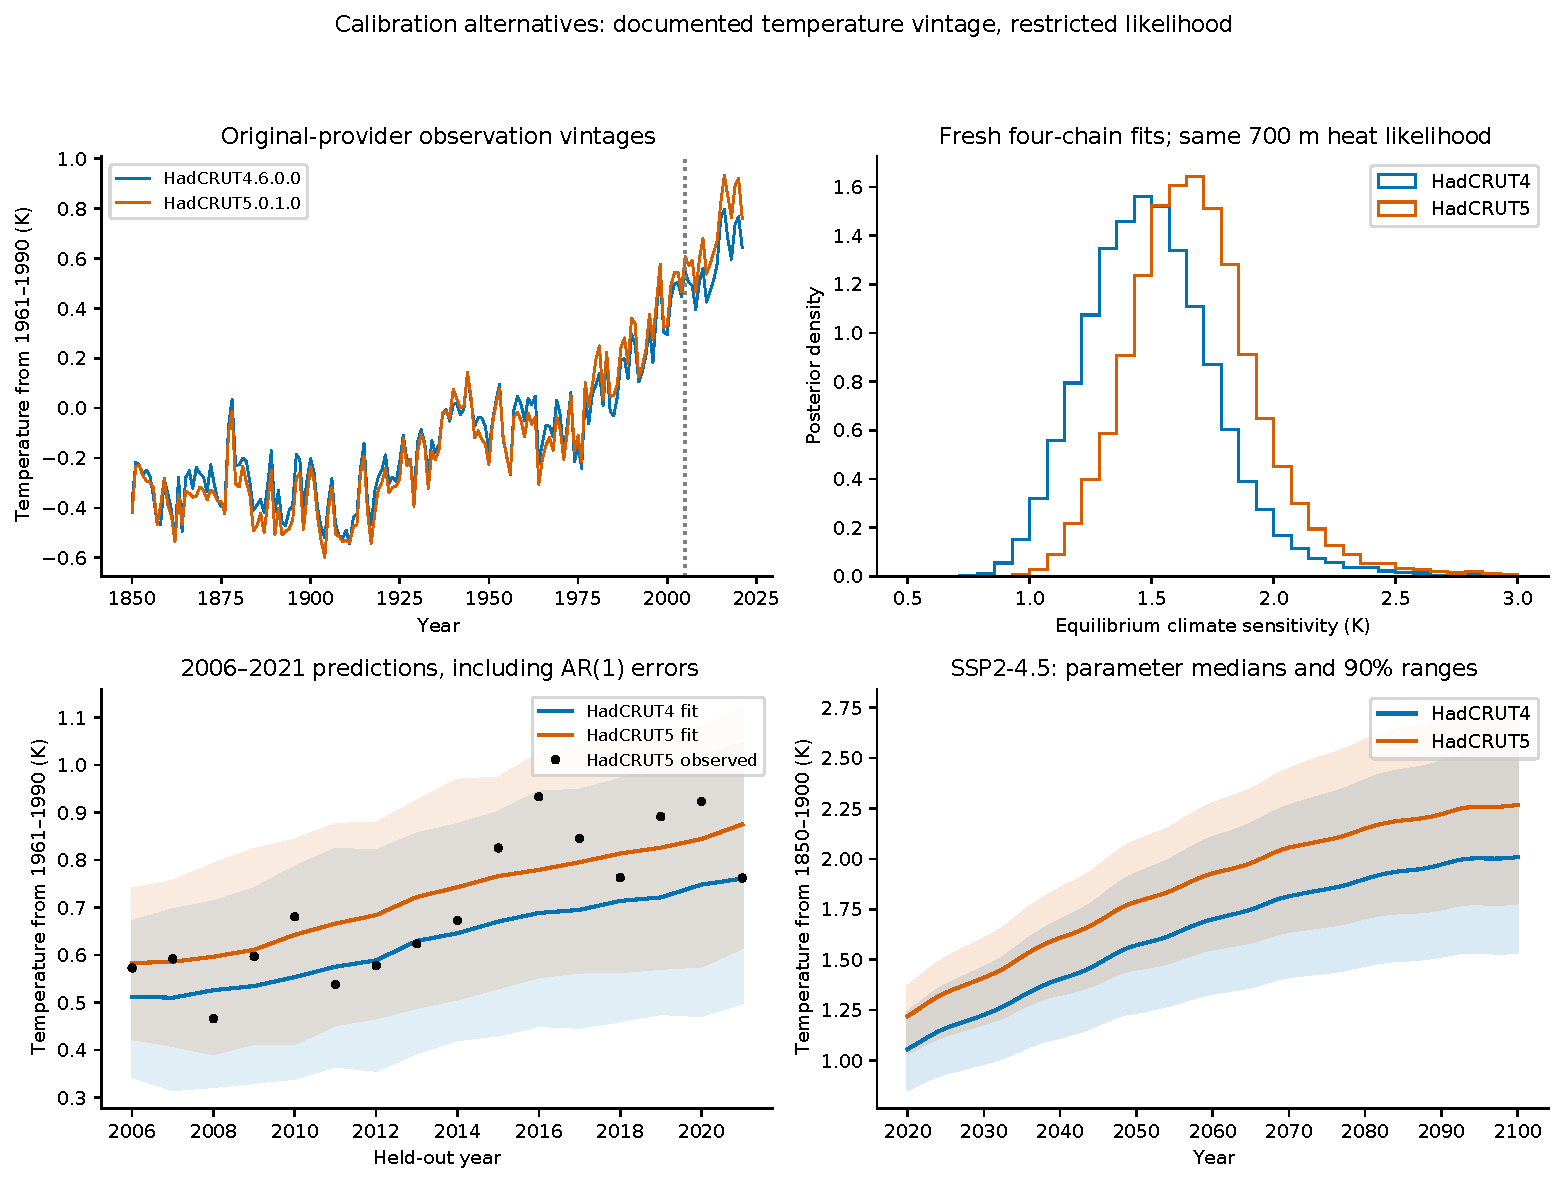
\includegraphics[width=\linewidth]{figures/observation_vintage_climate.pdf}
\caption{Observation-vintage alternatives. Upper left: original-provider
temperature records on their common 1961--1990 datum; the dotted line marks
the training cutoff. Upper right: independently sampled ECS posteriors under
the same 700 m heat constraint. Lower left: held-out temperature predictions
with stationary AR(1) errors and HadCRUT5 observations. Lower right: SSP2-4.5
parameter medians and 90\% ranges relative to each model's 1850--1900 mean.
The new fit changes the projection but does not recover the full target
calibration.}\label{fig:vintagetemperature}
\end{figure}

The written residual convention also motivates an observable-classification
test. Adding a stationary normal residual with variance
$\sigma^2/(1-\rho^2)$ to annual 2100 temperature gives an exact Gaussian-mixture
probability for each warming category. Under the 50\% budget weights, the
four probabilities change from 58.815/33.350/7.781/0.0534\% to
59.424/32.933/7.571/0.0724\%. This is an observation-error alternative:
the residual does not drive carbon or ice dynamics, and no sea-level residual
is silently added. It therefore tests classification separately from physical
climate response.

\subsection{Carbon constraints that fail to transfer}
The initial atmospheric CO$_2$ and fertilization coefficient are fitted under
the documented bounds 275--295 ppm and 0--1. The chemical reference equilibrium
is recomputed at each initial concentration. Temperature sensitivity of
respiration and thermocline exchange remain fixed at $Q_{10}=2$ and
16.87 m yr$^{-1}$. An initial noise-free recovery case passes, but the subsequent audit below
shows that this does not establish optimizer convergence on real data.
Zero-forcing and driven-mass tests verify the changed reference chemistry.
The combined observational objective gives equal weight to the mean squared
Mauna Loa and Law Dome residuals. This weighting is an explicit alternative,
not the recovered target likelihood. It also omits the documented ice-core
gas-age smoothing and dating uncertainty.

The original Mauna Loa-only fit reaches the lower initial-CO$_2$ bound and has a held-out
RMSE of 1.79 ppm. Adding Law Dome reduces its early-record RMSE from 7.91 to
1.99 ppm but increases the held-out Mauna Loa RMSE to 4.59 ppm. Substituting
HadCRUT5 gives a similar 4.19 ppm held-out error. Halving the integration step
changes CO$_2$ by at most $2.13\times10^{-4}$ ppm and carbon mass closes within
$3.64\times10^{-12}$ Gt C. The observational discrepancy is therefore much
larger than the tested temporal error. These restricted fits are retained as
failed predictive experiments and are not substituted into the coastal runs.

\begin{figure}[htbp]
\centering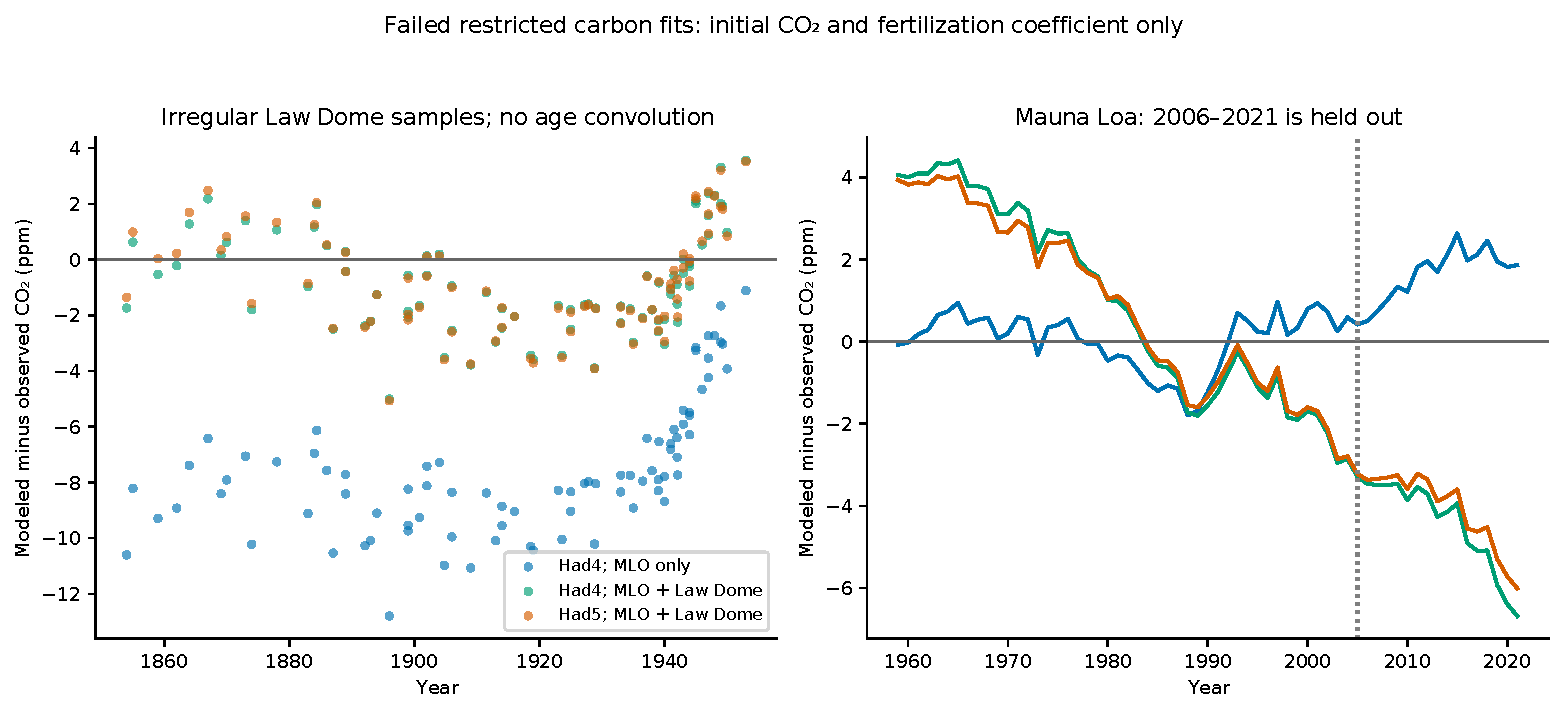
\includegraphics[width=\linewidth]{figures/observation_vintage_carbon.pdf}
\caption{Original restricted carbon fits against independently acquired observations.
Left: residuals at each irregular Law Dome gas age. Right: annual Mauna Loa
residuals, with 2006--2021 held out beyond the dotted line. The combined fits
improve the early record while degrading later predictions. The initial noise-free check passed, but later constrained-solver audits below
distinguish computational limitations from predictive discrepancies. Numerical
convergence alone cannot establish observational validation.}
\label{fig:vintagecarbon}
\end{figure}
The first attempt to fit $Q_{10}$ and thermocline transfer as additional
coordinates failed an internal nested-model check: a clipped Gauss--Newton
search stopped prematurely with training error above the restricted fit.
Those trajectories and searches are preserved as failed computations. A second,
bound-aware damped solver passes six analytic and nonlinear checks and includes
the restricted fit as a starting point. Nevertheless, its real-data pilot
reaches 100 iterations with projected gradient 0.0437 and objective 10.0613.
This is an unconverged computation, not evidence for the fitted physics. The
pilot is retained separately and its unfinished full run is interrupted.
We therefore also evaluate the unchanged Julia residuals using the installed
SciPy 1.5.4 bounded trust-region least-squares routine\cite{scipy15}. A pipe
passes parameter and residual vectors; the library imports no climate-model
implementation. Six cross-language tests check constrained analytical solutions
and a nonlinear valley. Synthetic parameter recovery and comparison with the
nested restricted model are required again before scientific interpretation.
Four starting points test local-solution dependence without proving a global
optimum. The objective contains no held-out data or target-figure values.

Repeated carbonate roots dominate residual evaluation. We add an optional
safeguarded Newton solution of the same equilibrium equation, retaining
bisection as the default. Write $x=\log H$, $y=K_1/H$ and $z=K_1K_2/H^2$,
where $H$ is hydrogen concentration and $K_1,K_2$ are dissociation constants.
If $M$ is combined atmosphere--mixed-ocean carbon, atmospheric concentration is
\begin{equation}
 C=\frac{M}{A+B(1+y+z)},\qquad
 \frac{dC}{dx}=\frac{CB(y+2z)}{A+B(1+y+z)}.
\end{equation}
Here $A$ converts atmospheric concentration to carbon and $B$ combines mixed-
ocean volume and solubility. Differentiating the existing alkalinity residual
then supplies the Newton step; steps outside the log-hydrogen bracket are
bisected. This changes the root algorithm, not the physical closure.
The absolute alkalinity tolerance is $10^{-16}$ mol/L. Across 102 tests,
isolated roots, mass/alkalinity balances and three historical integrations
agree with bisection. The central 172-year benchmark differs by
$7.43\times10^{-11}$ ppm in CO$_2$ and $3.28\times10^{-11}$ Gt C in stocks,
with about sevenfold local speedup. The unfinished slower free-fit pilot is
interrupted after this equivalence check; completed restricted bisection fits
and all failure records are preserved.


\subsection{Audited carbon fits and predictive disagreement}
The SciPy pilot passes noise-free four-parameter recovery to
$3.2\times10^{-11}$ in scaled coordinates. The full experiment completes all
twelve searches in 202 s, with no evaluation-limit stops. Three-point derivatives,
Jacobian scaling and objective/step tolerances of $10^{-10}$ are recorded;
the largest reported projected gradient is $1.55\times10^{-4}$. These are
objective-based local stopping conditions, not a claim that every coordinate
satisfies a $10^{-10}$ gradient criterion. Each selected training objective is
below its corresponding re-audited restricted value. Replaying all twelve
solutions verifies their objectives, agreement with bisection within
$1.05\times10^{-10}$ ppm, and time-step differences below
$1.91\times10^{-4}$ ppm. Selected fits conserve carbon within
$3.96\times10^{-12}$ Gt C.

Allowing respiration and thermocline transfer to vary improves the Mauna
Loa-only held-out RMSE from 1.738 to 0.858 ppm, but its initial concentration
remains at the 275 ppm lower bound (Table\ref{tab:carbonfree}). Adding Law Dome
retains different predictive behavior: HadCRUT4 combined RMSE rises from 4.589
to 6.193 ppm and HadCRUT5 combined RMSE from 4.185 to 4.330 ppm. The best
combined fits improve early-record RMSE to 1.736 and 1.979 ppm. Thus, lower
training error does not resolve transfer to the later observational period.
The likelihood weighting, gas-age mapping, initial disequilibrium and structural
response remain distinct scientific questions.

\begin{table}[htbp]\centering\small
\begin{tabular}{lrrrrrr}\toprule
Fit & $C_0$ & $\beta$ & $Q_{10}$ & Exchange & CO$_2$ RMSE & Ocean uptake\\
 & ppm & & & m/yr & ppm & Gt C\\\midrule
Had4, MLO & 275.000 & 0.431 & 1.529 & 21.867 & 0.858 & 143.161 \\
Had4, combined & 282.899 & 0.721 & 1.064 & 11.313 & 6.193 & 94.417 \\
Had5, combined & 284.121 & 0.944 & 1.897 & 8.572 & 4.330 & 78.319 \\

\bottomrule\end{tabular}
\caption{Selected conditional carbon point fits. CO$_2$ RMSE uses withheld
2006--2021 observations; ocean uptake is modeled from the 1850 initial state
to 1994. The Mauna Loa-only initial concentration reaches its lower bound.
These are fitted alternatives, not a target posterior or identified constants.}
\label{tab:carbonfree}
\end{table}

The starting-point audit also exposes weak discrimination among physical
responses. A second HadCRUT4 combined solution reaches the 200 m/year exchange
bound, with objective 10.0805 instead of 10.0613, a difference of only 0.19\%.
Its modeled 1994 ocean uptake is 196.95 Gt C, compared with 94.42 Gt C for the
selected minimum, while held-out RMSE is 6.011 instead of 6.193 ppm. Selection
uses the training objective throughout; held-out error is not used to choose a
basin. The written $118\pm19$ Gt C inventory has a different preindustrial
reference and is contextual evidence, not a matched likelihood or definitive
rejection test. These differences prevent interpreting a stable minimum from
several starts as a uniquely inferred carbon partition.

\begin{figure}[htbp]
\centering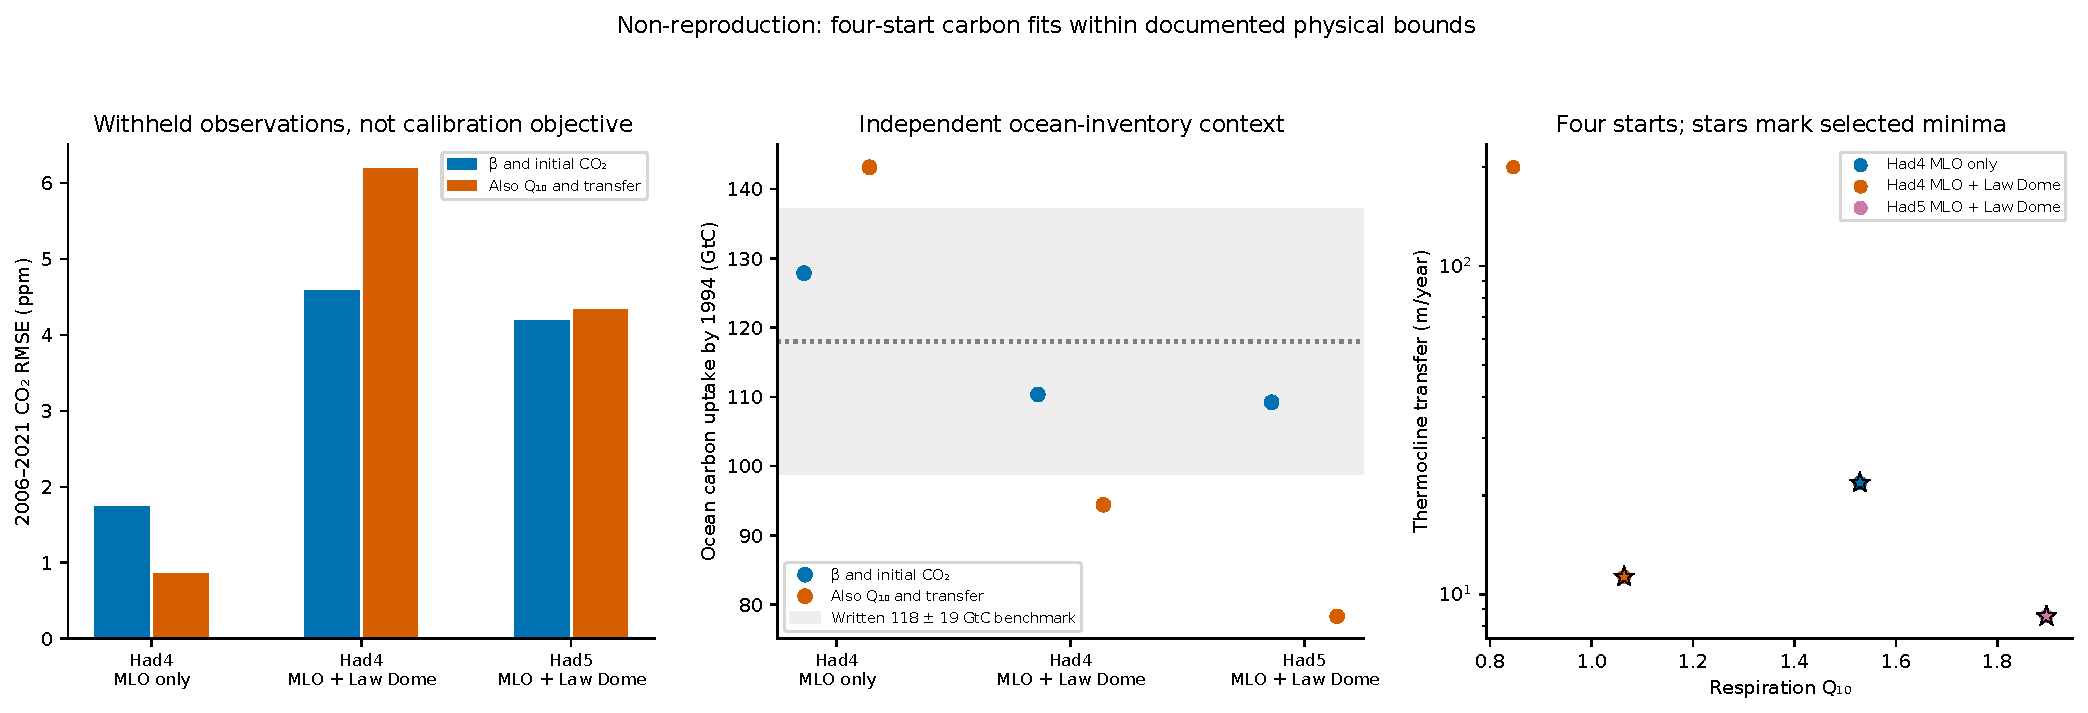
\includegraphics[width=\linewidth]{figures/carbon_parameter_sensitivity.pdf}
\caption{Audited carbon-parameter alternatives. Left: withheld CO$_2$ errors
for restricted and four-parameter fits. Center: selected ocean uptake compared
with the written inventory, whose time origin differs. Right: respiration
and transfer values from all four starts; stars mark selected training minima.
The alternative exchange-bound solution illustrates local-solution dependence.
None of these fits replaces the carbon point parameters in the coastal ensembles.}
\label{fig:carbonparameter}
\end{figure}

\subsection{An original-provider glacier record and a version discrepancy}
The NSIDC archive supplies a 2005 observational supplement to Dyurgerov's
glacier compilation \cite{nsidcglaciers}. Its Appendix 6 contains 43 annual
global sea-level contributions for 1961--2003. We extract spreadsheet cells,
verify annual-to-cumulative closure exactly, and cross-check the two populated
worksheets. No figure is digitized. The global columns agree even though some
regional entries differ. No annual global uncertainty column is supplied.

This archive is not confirmed identical to the cited Dyurgerov--Meier
Occasional Paper 58. Its mean is 0.404 mm/year for 1961--2003 and 0.723 mm/year
for 1994--2003, whereas the report's INSTAAR abstract states 0.51 and
0.93 mm/year. The old institutional download failed certificate validation, an earlier
current link returned 404, and the government archive timed out. A subsequent
search recovered the correctly capitalized institutional PDF URL; the printed
observations are evaluated separately below. The NSIDC values remain unchanged.

A conditional least-squares experiment fits the glacier temperature sensitivity
over 1961--1995 for 27 combinations of the documented volume, exponent and
initial-state bounds, separately using HadCRUT4 and HadCRUT5 temperatures.
The initial-state origin is explicitly assigned to 1961, and the observed
annual increments are associated with intervals beginning in their labeled
year. These choices, the rate objective and the absence of a joint AR(1)
calibration make the experiment an alternative. A noise-free scalar fit
recovers its known sensitivity to $4.4\times10^{-18}$ m/(K year).

The selected HadCRUT4 fit has sensitivity $6.70\times10^{-4}$ m/(K year)
and withheld 1996--2003 RMSE 0.228 mm/year; the HadCRUT5 fit gives
$6.10\times10^{-4}$ and 0.241 mm/year. Both outperform a trend estimated
from the same training years, whose withheld RMSE is 0.355 mm/year.
The training minima occur on volume, exponent and initial-state grid boundaries;
we do not interpret them as identified physical parameters or a global optimum.
Comparison with GlaMBIE in 2004--2020 gives RMSE 0.230 and 0.220 mm/year,
but the observation products have different spatial coverage. They differ by
0.389 mm/year RMS during their four overlapping years. No fitted parameters
from this sensitivity replace the accepted coupled sea-level calculations.

\begin{figure}[htbp]
\centering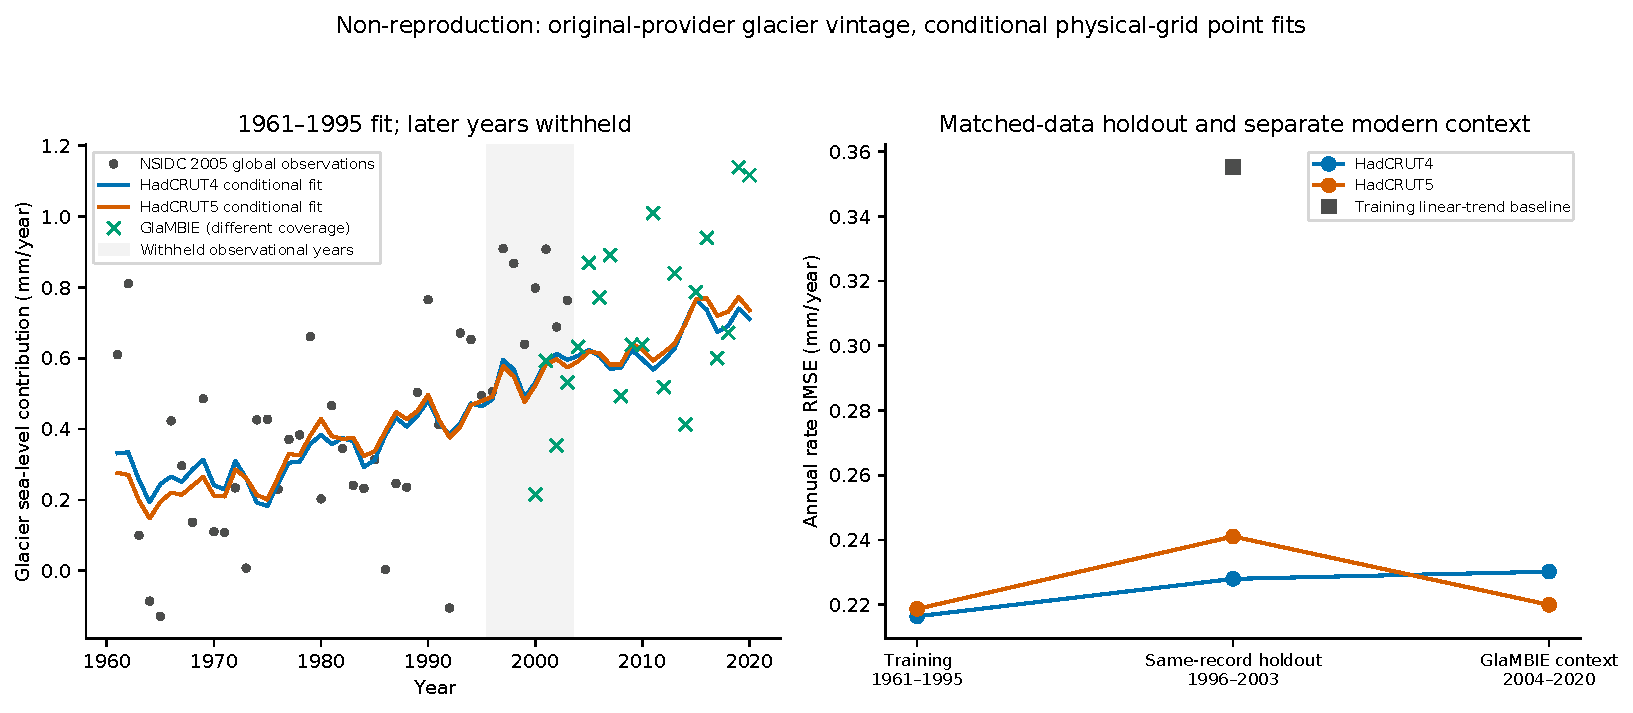
\includegraphics[width=\linewidth]{figures/glacier_observation_vintage.pdf}
\caption{Glacier observation-vintage test. Gray points are the original NSIDC
spreadsheet observations; colored lines are independently fitted conditional
model rates. The shaded interval is withheld from fitting. Crosses show the
newer GlaMBIE observations, which have different coverage. Right: training
and withheld errors, with the later product treated as separate context.
The archived NSIDC series differs from the cited report's written average;
this is a non-reproduction.}
\end{figure}

\subsection{Recovery of the cited glacier report}
The institutional OP58 report is now available at a correctly capitalized URL
\cite{op58}. Appendix 3, printed page 117, supplies annual global observational
SLR increments and cumulative values for 1961--2003. Text-table extraction gives
means of 0.511 and 0.927 mm/year over the two stated intervals. Annual increments
and cumulative values are independently rounded to 0.01 mm, so individual
closure discrepancies reach 0.01 mm. We preserve that rounding and verify it
against the printed volume conversion; no figure is digitized. The source
includes peripheral glaciers and supplies no annual global uncertainty column
in this table. Recovering it therefore resolves the unavailable-record claim,
while leaving the target likelihood, processed input identity and component
coverage conventions to be established.

Repeating the same conditional 54-point glacier experiment on this record gives
HadCRUT4 and HadCRUT5 sensitivity estimates of $8.25\times10^{-4}$ and
$7.52\times10^{-4}$ m/(K year). The withheld 1996--2003 rate RMSE is
0.400 and 0.412 mm/year, compared with 0.578 for the training linear trend.
The selected physical grid points again lie on all three boundaries. Their
2004--2020 GlaMBIE contextual RMSE is 0.201 and 0.202 mm/year, with unmatched
coverage. The original observational products differ by 0.730 mm/year RMS in
2000--2003. This is a reproducible observation-version comparison, not a fitted
error bar or recovery of the target glacier posterior.

\begin{figure}[htbp]
\centering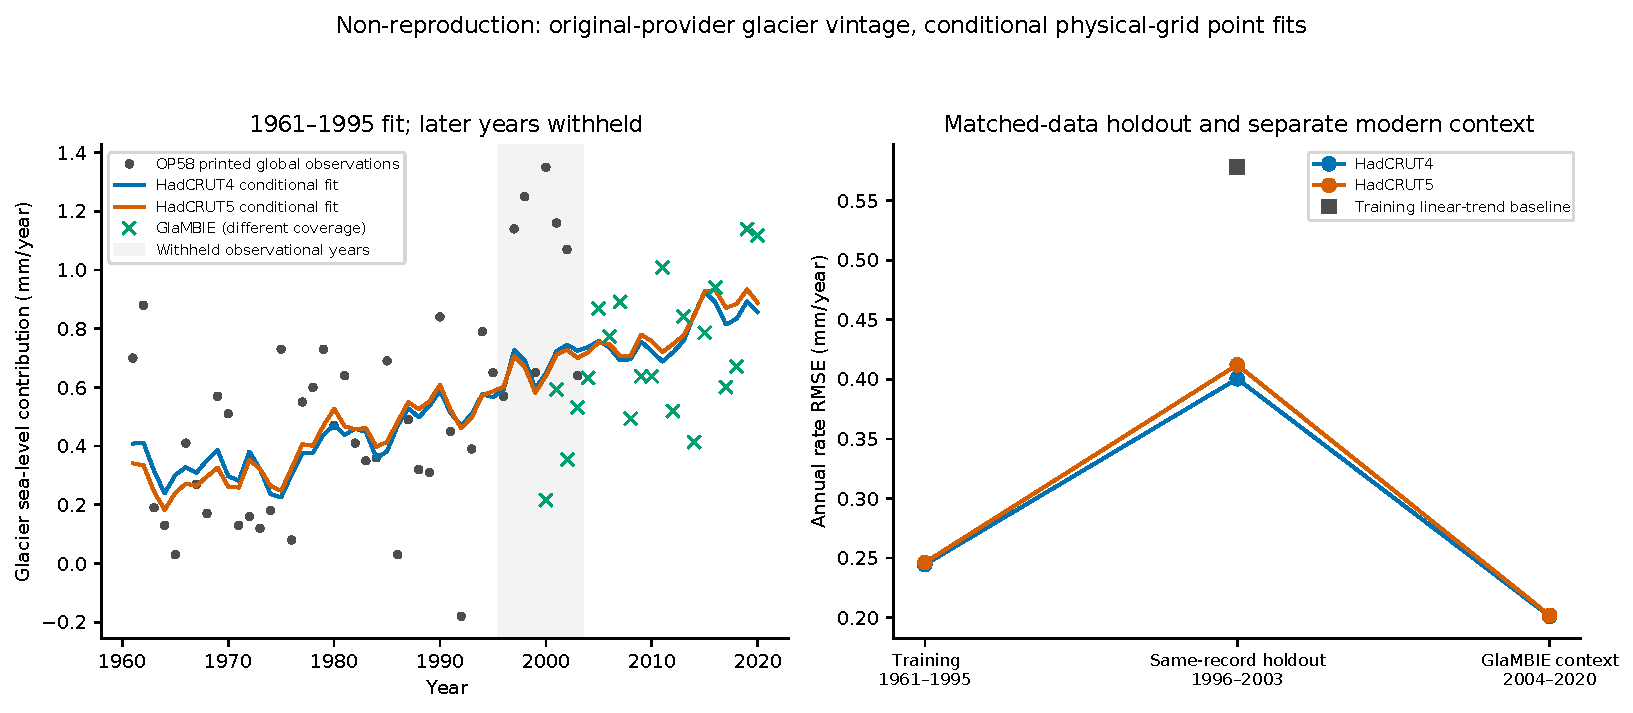
\includegraphics[width=\linewidth]{figures/glacier_op58_fit.pdf}
\caption{Conditional glacier fit using the recovered OP58 printed observations.
The same grid, training boundary and withheld years as the NSIDC experiment
isolate the source-version change. The later GlaMBIE record is separate context.
No fitted glacier parameters in this figure replace the base sea-level ensemble.}
\end{figure}
\subsection{Propagation of the temperature-version change}
The independently calibrated HadCRUT5 posterior now drives 250 emissions states
and 2,500 sea-level cases under the same five closure choices and two non-CO$_2$
rules. Its pilot checks give maximum CO$_2$ and temperature differences of
$4.82\times10^{-4}$ ppm and $9.05\times10^{-6}$ K when halving the step;
Antarctic refinement differs by $2.45\times10^{-13}$ m. The carbon hindcast and
point parameters remain fixed so that these runs isolate the posterior change.

Under the explicit 50\% budget-event weights, median annual 2100 warming rises
from 1.264 to 1.484 K. Its 5th--95th range changes from 0.838--2.606 K to
0.996--2.879 K. The corresponding median uncorrected sea-level rise from 2010
changes from 0.232 to 0.237 m, while its upper percentile rises from 0.641 to
0.736 m. The fixed Antarctic model's triggering probability rises from 13.99\%
to 18.77\%. Category counts become 101, 56, 71 and 22; their weighted masses
are 54.59, 34.26, 10.76 and 0.393\%. These are conditional alternatives, not
estimates under the recovered expert-density likelihood or the target posterior.
The additional high-warming states motivate a separately validated coastal
propagation rather than assuming that the earlier cost distribution transfers.

\subsection{Separating heat constraints from expert-emissions assumptions}
The temperature-only posterior supplies a third, deliberately unfavorable
predictive comparison. We propagate the same 250 emissions states through
each independently sampled climate posterior, holding carbon and ice choices
fixed. Parameter values are not paired between posteriors; only the emissions
design and random row indices are shared. Figure\ref{fig:climateconstraints}
therefore compares distributions, not the response of a single physical state
to changing an observation.

Omitting the upper-ocean heat constraint raises median annual 2100 warming
under the 50\% budget-event alternative to 2.156 K, with a 5th--95th range of
1.261--3.935 K. Warming-category counts are 25, 84, 63 and 78, with weighted
masses 13.02, 47.39, 29.71 and 9.87\%. The corresponding uncorrected sea-level
median is 0.450 m from 2010, with range 0.244--1.423 m, and the fixed Antarctic
fast-loss model activates in 43.91\% of weighted paths. The high-category mass
is closer to the target's printed 7.78\% than either heat-constrained result.
However, this posterior has withheld temperature RMSE 0.209 K, bias
$+0.189$ K and upper-ocean heat RMSE $16.46\times10^{22}$ J. Its failure to
predict these independent observations prevents using category resemblance
to select it as a recovered calibration.

The three climate ensembles pass the same time-step and carbon-accounting
checks. The temperature-only pilot's maximum changes are
$5.10\times10^{-4}$ ppm CO$_2$ and $8.98\times10^{-6}$ K; carbon mass closes
within $1.28\times10^{-11}$ Gt C over the full ensemble. Thus, these distribution
differences exceed the measured numerical time-step effects. The experiment
tests the influence of an alternative 700 m constraint. It does not recover the
missing annual 3000 m observational record.

\begin{figure}[htbp]
\centering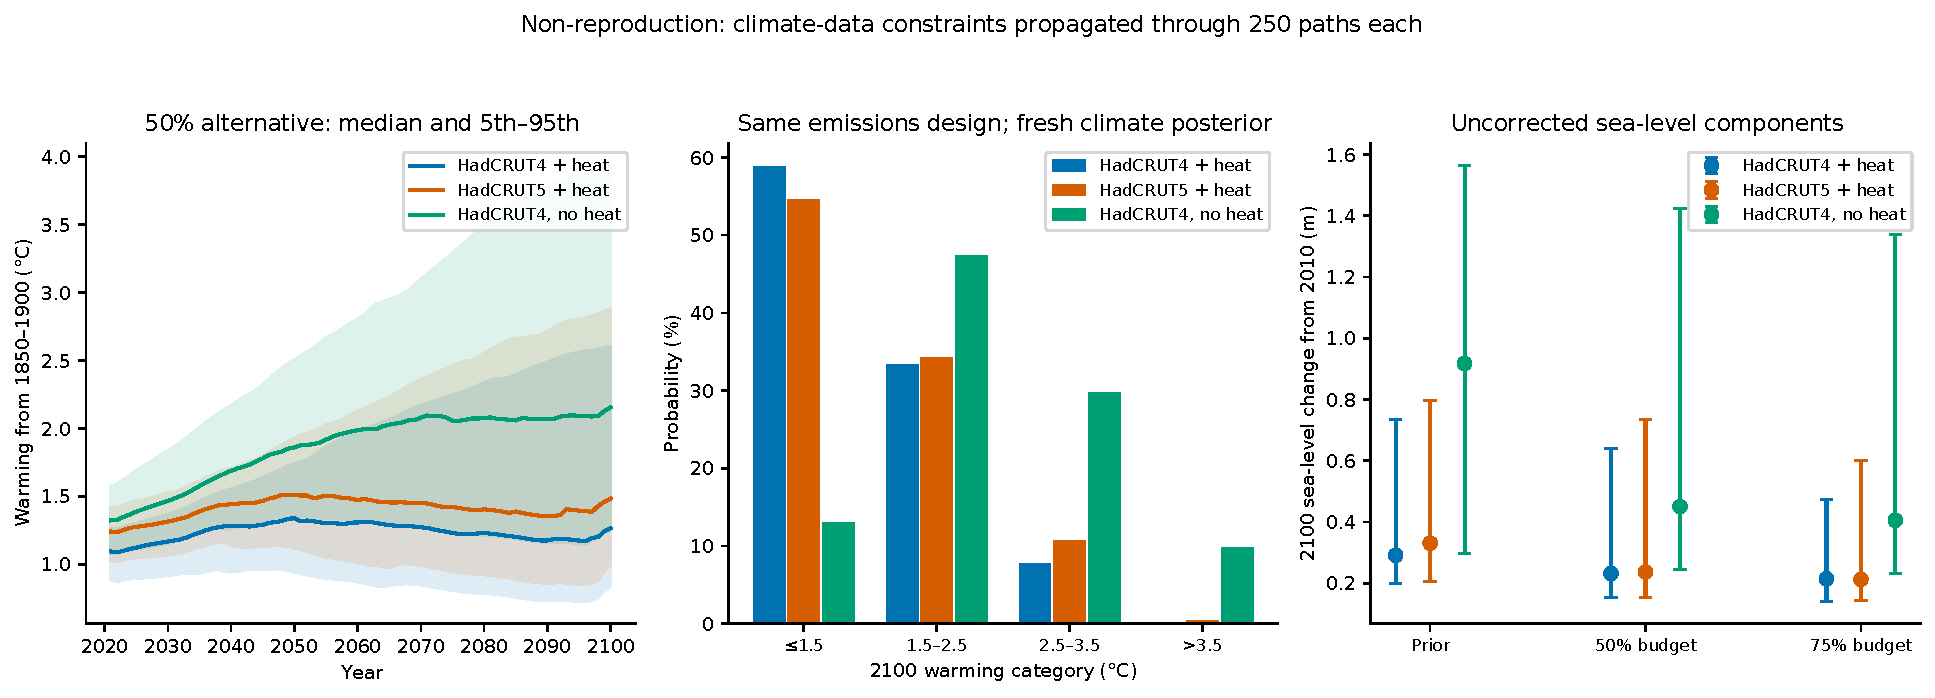
\includegraphics[width=\linewidth]{figures/coupled_climate_vintage_sensitivity.pdf}
\caption{Climate-observation constraints propagated through independent
emissions-driven alternatives. Left: annual warming medians and 5th--95th
percentiles under explicit 50\% budget-event weights. Center: 2100 category
masses under those weights. Right: uncorrected global sea-level medians and
5th--95th percentiles under three alternative emissions measures, relative to
2010. Colors distinguish independently calibrated climate posteriors. The
temperature-only result fails predictive checks; none is the target posterior.}
\label{fig:climateconstraints}
\end{figure}

Applying the recovered prior-times-expert-density inversion changes the
distributions again (Figure\ref{fig:expertdensityclimate}). Across the four
explicitly assumed densities, HadCRUT4 with heat gives only
0.0072--0.0399\% probability above 3.5 K; HadCRUT5 with heat gives
0.193--0.450\%. Temperature-only fits give 17.09--18.09\%, despite all four
expert densities assigning the same 50\% mass to the cumulative-emissions
budget event. Median sea-level changes range from 0.277--0.291 m,
0.321--0.334 m and 0.867--0.903 m, respectively. These are different likelihood
assumptions from directly imposing a posterior budget-event probability. The
spread identifies two consequential unresolved choices: the climate likelihood
and the complete expert density. It supplies no basis for choosing either to
force a match to the target.

\begin{figure}[htbp]
\centering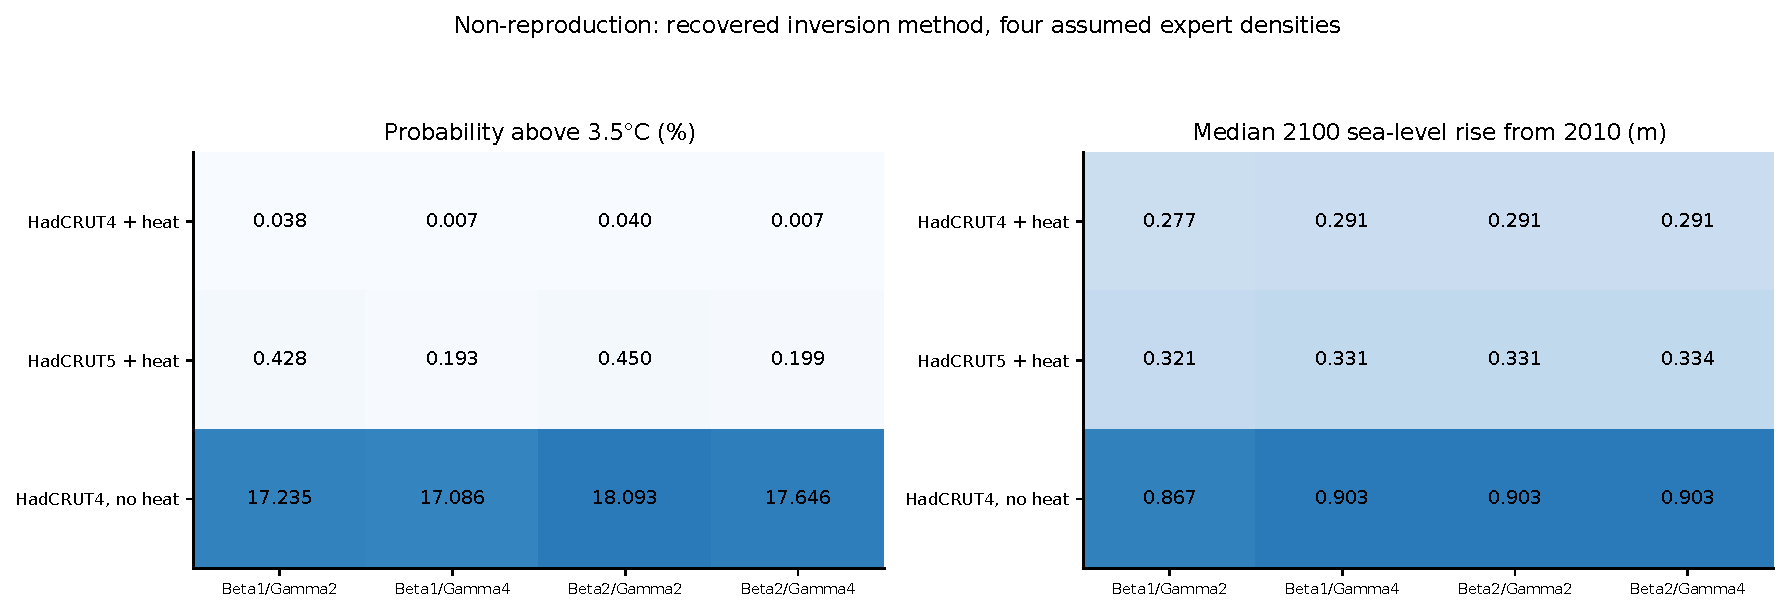
\includegraphics[width=\linewidth]{figures/coupled_expert_climate_sensitivity.pdf}
\caption{Recovered inversion method with four alternative expert probability
densities and three independent climate calibrations. Entries show probability
above 3.5 K and median uncorrected sea-level change from 2010. The lower-budget
density is uniform or Beta(2,2); the upper-budget tail uses Gamma shape two or
four, with the documented conditional mode and budget mass imposed. The
families and widths are assumptions. No target posterior is inferred from this
comparison.}
\label{fig:expertdensityclimate}
\end{figure}

For comparison with the target's reference period, each sea-level member is
also shifted by its own modeled 1995--2014 arithmetic mean. Under 50\%
budget-event weights the HadCRUT5 median becomes 0.250 m, with 17th--83rd
percentiles 0.193--0.457 m. The temperature-only median becomes 0.465 m,
with interval 0.322--1.178 m. The datum corrections are 0.0065--0.0180 m and
0.0119--0.0262 m across the five closure alternatives. These shifts reconcile
reference periods only; they do not make the emissions ensemble commensurate
with an individual AR6 SSP scenario or remove component-coverage overlap.
